\section{Auswertung}
\label{sec:Auswertung}

\subsection{Fourier-Synthese}
\noindent Bei der Furier-Synthese Wurde versucht eine 
Sägezahnspannung, eine Rechteckspannung und eine Dreiecksspannung 
darzustelllen. 
\noindent Wenn die Spannungen an den vielfachen der Grundfrequenz mithilfe des 
Oberwellengenerators so eingestellt werden Kommen die folgenden Furier-Reihen dabei raus.
\begin{figure}[H]
    \centering
    \caption{Furier-Reihe Sägezahnspannung}
    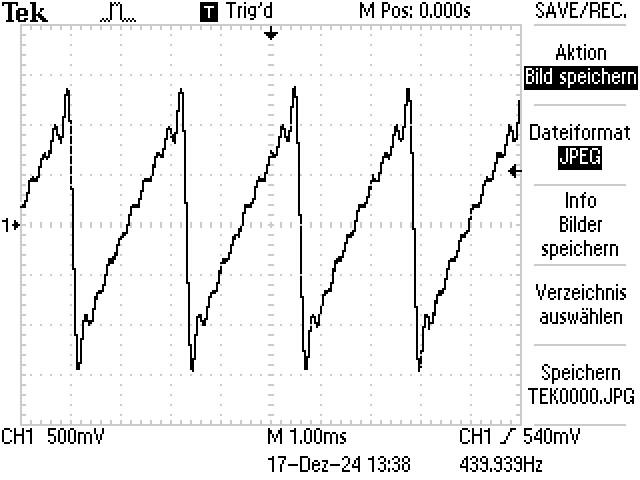
\includegraphics{Bilder/TEK0000.JPG}
\end{figure}

\begin{figure}[H]
    \centering
    \caption{Furier-Reihe Rechteckspannung}
    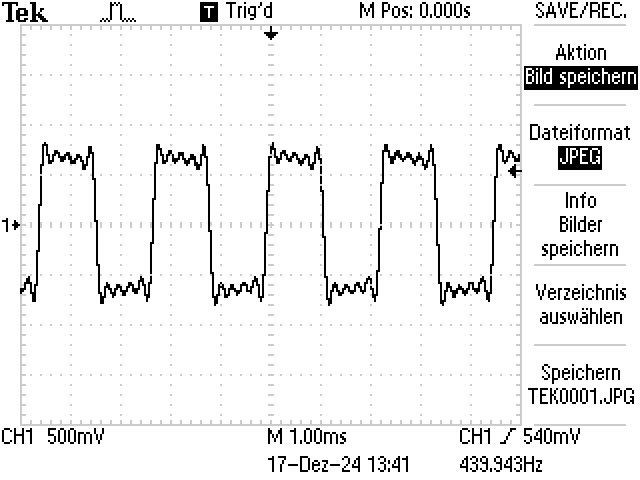
\includegraphics{Bilder/TEK0001.JPG}
\end{figure}

\begin{figure}[H]
    \centering
    \caption{Furier-Reihe Dreieckspannung}
    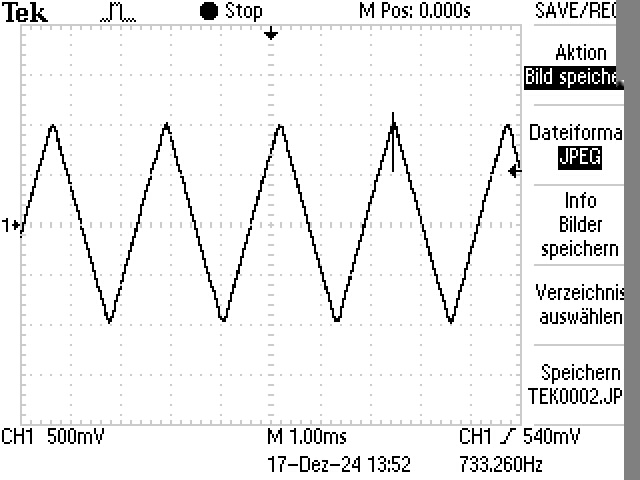
\includegraphics{Bilder/TEK0002.JPG}
\end{figure}


\subsection{Fourier-Analyse}
Bei der Fourier-Analyse werden am Oberwellengeneratur die Rechtecksfunktion,
die Dreiecksfunktion und die Sägezahnfunktion generiert. Am Amperemeter werden 
die Amplituden bei den jewailigen Frequenzen der Oberwelle abgelesen, um so
auf die Abhängigkeit der Spannung der $n$-ten Oberwelle von $n$ schließen zu
können.
\subsubsection{Rechteckspannung}
\begin{table}[H]
    \centering
    \caption{Amplituden der Oberschwingungen Rechtecksfunktion.}
    \label{tab:j1}
    \begin{tblr}{
        colspec = {S S S},
        row{1} = {guard, mode=math},
      }
    \toprule
    f (\unit{\hertz}) &  A (\unit{\deci\bel})\\
    \midrule
    10 & 17.8\\
    30  & 9.01\\
    50  & 4.61\\
    70  & 1.81\\
    90  &-0.19\\
    110 &-1.79\\
    130 &-3.39\\
    150 &-4.59\\
    170 &-6.19\\
    190 &-8.19\\
    \bottomrule
    \end{tblr}
\end{table}
\noindent Die Oberwellen sind jewils die n-mal vielfachen der Grundfrequenz
Um auf die Abhängigkeit von n schließen zu können, fitten wir die 
in Volt umgerechneten Spannungswerte die gegen die ordnung der jewailigen 
Oberwelle aufgetragen sind an eine Funktion der Form 
\begin{equation}
    \label{eqn:1}
    U(n) = \frac{a}{n^b}
\end{equation}
\noindent Die umrechnung in Volt wird auf grundlage der Proportionalität $\unit{\volt} \tilde e^{\frac{\unit{\decibel}}{20}}$ ausgeführt.




\begin{figure}
    \centering
    \caption{Curve Fit und Messwerte Rechteckspannung}
    \includegraphics{viereck.pdf}
\end{figure}

\noindent aus dem Curve fit mithilfe der Python Bibiliothek "Pyplot" erhalten wir 
für die Rechtecksspannung die Paarameter 
\begin{align*}
    a = & \num{7.7 +- 1.0}\\
    b = & \num{1.34 +- 0.26}\\
\end{align*}
\noindent Der Ausgleichsparameter $b$ gibt und somit den Grad der abhängigkeit von n an.



\subsubsection{Dreieckspannung}
\begin{table}[H]
    \centering
    \caption{Amplituden der Oberschwingungen Dreiecksfunktion.}
    \label{tab:j1}
    \begin{tblr}{
        colspec = {S S S},
        row{1} = {guard, mode=math},
      }
    \toprule
    f (\unit{\hertz}) &  A (\unit{\deci\bel})\\
    \midrule
    10  & 14.2  \\
    30  & -4.59 \\
    50  & -13.4 \\
    70  & -19.4 \\
    90  & -23.4 \\
    110 & -27.0 \\
    130 & -29.4 \\
    \bottomrule
    \end{tblr}
\end{table}
\noindent Auch bei der Dreiecksspannung wird ein Curf fit durch eine Funktion der Form
aus \autoref{eqn:1} auf die Messdaten angewendet. 

\subsubsection{Dreiecksfunktion}
\begin{figure}[H]
    \centering
    \caption{Curve Fit und Messwerte Dreiecksspannung}
    \includegraphics{dreieck.pdf}
\end{figure}

\noindent Die Parameter a und b ergeben sich zu 
\begin{align*}
    a = & \num{5.1 +- 1.0}\\
    b = & \num{3.0 +- 2.1}\\
\end{align*}
\noindent Wobei b wieder den grad der n abhängigkeit angibt.


\subsubsection{Sägezahnspannung}
\begin{table}[H]
    \centering
    \caption{Amplituden der Oberschwingungen Sägezahnfunktion.}
    \label{tab:j1}
    \begin{tblr}{
        colspec = {S S S},
        row{1} = {guard, mode=math},
      }
    \toprule
    f (\unit{\hertz}) &  A (\unit{\deci\bel})\\
    \midrule
    10  & 11.8  \\
    20  &  7.01 \\
    30  &  3.01 \\
    40  &  1.01 \\
    50  & -1.39 \\
    60  & -2.99 \\
    70  & -4.00 \\
    80  & -5.79 \\
    90  & -6.19 \\
    100 & -8.99 \\
    110 & -7.79 \\
    120 & -9.79 \\
    130 & -9.39 \\
    \bottomrule
    \end{tblr}
\end{table}


\subsubsection{Sägezahnfunktion}[H]
\begin{figure}
    \centering
    \caption{Curve Fit und Messwerte Sägezaahnspannung}
    \includegraphics{saege.pdf}
\end{figure}
\noindent Die Ausgleichsparameter für die Sägezahnspannung lauten
\begin{align*}
    a = & \num{4.0 +- 0.9}\\
    b = & \num{0.94 +- 0.28}\\
\end{align*}


%Auskommentiert, da es irgendwie Probleme mit "\includegraphics{rechteck.pdf}"
%gab (bereits bei make nachdem ich direkt gepullt habe)



